\graphicspath{{Chapters/SCT/Figures/}}
% 1/4/2010 - 13/10/2012
% T diff slope =  1.2827722385  +/- 0.190113543082
% #Delta T slope =  0.884557428732  +/- 0.0636293102113
\def\NumHighDeltaTModulesIncreaseRate{1.28 \ensuremath{\pm} 0.19}
\def\NumHighTdiffModulesIncreaseRate{0.88 \ensuremath{\pm} 0.06}


\chapter{ATLAS Semiconductor Tracker Temperature Monitoring}
\label{chap:SCT}

\section{Introduction}

An overview of the Semiconductor Tracker (SCT) is given in
Section~\ref{sec:Detector-SCT}. In order to mitigate the effects of radiation
damage, it is necessary to keep the SCT modules at a temperature of around $-7
\circ C$; this is discussed in more detail below. An evaporative cooling system
has been put in place to achieve this; this is described in Section ?.

In order to monitor the performance of the cooling system, the temperature of
each SCT module is monitored by a thermistor mounted on the front side of the
detector (the side furthest from the interaction point). The barrel modules have
an additional thermistor mounted on the back side of the module. Monitoring of
the module temperature is important to ensure that the cooling system is
functioning as designed and that the modules are still coupled to the cooling
structures. The temperature difference between the front and the back of barrel
modules can be used to identify modules losing mechanical integrity. To this end
tools were developed to monitor variables associated with the temperatures of
SCT modules. These are described in this section, along with results for
twenty-two months of operation between January 2010 and October 2012.

\subsection{Effects of Radiation Damage on Semiconductor detectors}
Given the LHC design luminosity of $10^{34}$cm$^{-2}$s$^{-1}$, the
inner parts of the 
SCT are expected to receive a radiation dose of up to
$2x10^{14}\rm{n_{eq}/cm}^2$~\cite{Ahmad200798} over the course of it's desugn
lifetime of 10 years.
Exposure to such high radiation doses causes damage to the silicon detectors. 

The primary cause
of damage is interactions with irradiating particles displacing nuclei from
their lattice position. This can have the effect of removing donors, or of
creating acceptor like defects. Exposure to radiation will eventually cause an n-type
semi-conductor to become less heavily doped, and in extreme causes change the
material from n-type to p-type. Consequently, the displacement voltage required
to fully deplete the detector increases, and for sufficiently high radition doses it
becomes impossible to fully deplete the detector. It is therefor essential to
reduce the effects of radiation damage as much as possible.

The effects of exposure to radiation have both
an immediate and a prolonged effect. Immediate effects include the removal of
donor nuclei from the lattices, and creation of acceptor like defects. Due to the
complicated kinetics of these defects after the radiation, an annealing effect
occurs which initially reduces the number of acceptor-like defects, on a timescale of
approximately two days, but on a longer term a `reverse annealing' occurs,
increasing the number of acceptors. The rate of the reverse annealing effect is dependant on the temperate of the
silicon. It is found that for temperatures of approximately -7 $\circ C$ the
reverse-annealing effect is effectively frozen out~\cite{Lindstrom2001308}. Since the reverse annealing
occurs even after radiation, it is important to run the detector cooling at all
times, not just when particle collisions are occurring.

Lattice defects introduced as a result of exposure to radiation also causes an
increase of the leakage current, and
a loss of mobility,  both of which increases the level of noise in the detector. Since
the leakage current is induced by thermal creation of electron-hole pairs from
shallow donors, the size of the leakage current is also dependant on
temperature: 

\begin{equation}
I_{\rm{leakage}} (T) \propto T^{2} \rm{e}^{-\frac{E_{g}}{2k_{B}T}}
\end{equation}


\subsection{The SCT Cooling System}
Each SCT module currently produces between 5.5 and 6W of heat. This is expected
to increase to around 8W as the detector suffers the effects of radiation
damage. As described in the previous section, the silicon detectors must be run
at temperatures of around -7$^{\circ}$C in order to slow the rate of radiation
damage and prolong their lifetime. An active cooling system based upon
evaporative cooling is used to keep the modules at this temperature. This is
described in detail in~\cite{1748-0221-3-07-P07003}. C$_3$F$_8$ gas is delivered in liquid phase at -25 $^{\circ}$C to capillaries located immediately before the detector structure. The fluid expands through the capillaries and passes along a cooling pipe. The modules are coupled to the pipe by means of cooling blocks and heat is absorbed from the modules by the passing fluid causing it to evaporate. The exhaust gas is then compressed, cooled, and returned to the cooling loop.

\section{Methodology}
The temperatures recorded by the module thermistors are read out by the ATLAS \textit{PVSS} SCADA system. Twice a day the temperatures are written to an Oracle database for offline analysis. In addition, whenever a module temperature changes above a deadband of 0.4 $^\circ$C the new value is written to the database.
It is necessary to first find periods of stable running where the cooling system is turned on and the system in a stable state. Stable periods are found by requiring that the number of cooling loops turned on is constant and greater than zero. Stable periods are required to be at least 6 hours long, to veto periods where the detector is being turned on and off. Stable periods longer than 24 hours are broken down into 24 hour blocks.

For each module, a number of monitoring variables are calculated; these are described below. The distributions of these variables are plotted for each of the barrel layers and endcap disks. Modules which fall in the far outlying regions of the distributions are identified as `problem' modules. A list of problem modules is maintained, and these modules are monitored. The plots are produced automatically on a daily basis by scripts running on one of the SCT monitoring computers. The plots are made available as part of the `SCT Calibration Monitoring' website at \url{https://pc-sct-www01.cern.ch/CalibMonitor/} (ATLAS login required).

\section{Monitoring Variables}

\subsection{Front-Back temperature difference - \deltat }

SCT barrel modules have two thermistors, one mounted on either side of the module. The difference in temperature between the front and back of the module should be very small and any large temperature difference would indicate defective thermal coupling between the two sides. This would suggest that the front and the back of the module had lost mechanical integrity and were coming apart from one another. The monitoring variable \deltat is defined as

\begin{equation}
 \Delta T = T_{\mathrm{front}} - T_{\mathrm{back}}
\end{equation}

where $T_{\mathrm{front}}$ and $T_{\mathrm{back}}$ are the temperatures recorded at the front and the back of the module respectively. 

\begin{figure}[h]
\centering
\centering
\includegraphics[width=\textwidth]{{20120922.0120-20120923.0120_delta_t_AllBarrels}.pdf}
\caption{\deltat distribution for all SCT barrels averaged over the period 01:20 22/9/2012 to 01:20 23/9/2012. The distribution is fit to a Gaussian; the mean and width of the Gaussian is indicated on the plot.}
\label{fig:dt_dist}
\end{figure}

\begin{figure}[h]
	\centering
	\subfigure[]{
		\includegraphics[width=0.47\textwidth]{{20120922.0120-20120923.0120_delta_t_Barrel3}.pdf}
	}
	\subfigure[]{
		\includegraphics[width=0.47\textwidth]{{20120922.0120-20120923.0120_delta_t_Barrel4}.pdf}
	}
	\subfigure[]{
		\includegraphics[width=0.47\textwidth]{{20120922.0120-20120923.0120_delta_t_Barrel5}.pdf}
	}
	\subfigure[]{
		\includegraphics[width=0.47\textwidth]{{20120922.0120-20120923.0120_delta_t_Barrel6}.pdf}
	}
	\caption{\deltat distributions for the SCT Barrel 3 (a), Barrel 4 (b), Barrel 5 (c) and Barrel 6 (d) for 01:20 22/9/2012 to 01:20 23/9/2012. The distributions are fit to a Gaussian; the mean and width of the Gaussian is indicated on the plot.}
	\label{fig:dt_dist_barrels}
\end{figure}



For each period of stable operation the distribution of \deltat is plotted, for
all barrels together as well as for each barrel separately. Example plots for
01:20 22/9/2012 to 01:20 23/9/2012 are shown in Figure~\ref{fig:dt_dist} (all
barrels) and  in Figure~\ref{fig:dt_dist_barrels} (separately for each barrel).
The distributions are fitted with a Gaussian and the mean and width of the
Gaussian are obtained. These are listed in Table~\ref{table:dt_thresh} for each of the barrel layers, averaged over 5 months of data between 20/1/2010 and 20/6/2010.  

In order to identify modules with a high value of \deltat, a threshold of 5
times the width of the Gaussian is set, separately for each barrel. Modules with
a value of \deltat greater than the threshold are identified as `problem
modules'. Table~\ref{table:dt_num} gives the number and percentage of modules
with front-back temperature difference greater than the threshold at least five
times during the period 20/1/2010 - 19/6/2010 for each barrel layer. The width
of the distribution is greatest for Barrel 3, and so the thresholds for
identifying high \deltat modules is highest for this barrel. The width of the
distribution for Barrel 6 is the second widest, however the distribution is
observed to have large non Gaussian tails. Subsequently, the percentage of
modules falling outside of the Gaussian is far higher than for other barrels and
so a higher proportion of the modules on Barrel 6 are identified as problematic than on other barrels. This is explained by the fact that for Barrels 3, 4 and 5 only modules with $|\Delta \mathrm{T}| < 2^\circ$C measured on production were accepted, whereas for Barrel 6 this was relaxed to $|\Delta \mathrm{T}| < 4^\circ$C~\cite{Viehhauser:2006ix}. 

The mean value of the \deltat distributions tend to be negative, implying that on average the back side of the modules (the side facing into the carbon fibre barrel) tend to be warmer than the front. This effect was also observed in tests carried out on the modules reception at CERN in 2006~\cite{Viehhauser:2006ix}, and in tests carried out in 2008~\cite{Shaw:1229428}. Investigations suggested that this bias is a property of the module itself, rather than an effect due to the module's environment. A possible explanation is that the bend in the hybrid is on the back of the module, and this may have caused difficulties in manufacturing an  effective glue joint, increasing thermal impedance and causing a weaker thermal coupling between the cooling pipe and the back of the module.

\begin{table}
\centering
\begin{tabular}{ l | c  c  c  c }
\hline\hline
Barrel & $\sqrt{\langle \sigma ^ 2 \rangle }$ & $5\sqrt{\langle \sigma ^ 2 \rangle }$ & $\chi ^2 $  / ndf & $\langle \Delta T_{\mathrm{mean}} \rangle$ \\
\hline
All barrels & 0.52 & 2.61 & 132.64 & -0.25\\
Barrel 3 & 0.64 & 3.21 & 19.44 & -0.36 \\
Barrel 4 & 0.39 & 1.96 & 8.22 & -0.21 \\
Barrel 5 & 0.48 & 2.38 & 36.06 & -0.23 \\
Barrel 6 & 0.60 & 3.02 & 59.06 & -0.26 \\
\hline\hline
\end{tabular}
 \caption{The width, goodness of fit and mean of the Gaussian fit to the \deltat distribution averaged over stable periods between 20/1/2010 and 20/6/2010.}
	\label{table:dt_thresh}

\end{table}

\begin{table}
\centering
 \begin{tabular}{  l | c  c }
\hline\hline
Component & \# Problem Modules & \% Modules Problematic \\
\hline
Barrel 3 & 1 & 0.3 \\
Barrel 4 & 1 & 0.2 \\
Barrel 5 & 7 & 1.2 \\
Barrel 6 & 17 & 2.5 \\
\hline\hline
\end{tabular}
\caption{Number and percentage of modules with $|$ \deltat$|$ greater than the threshold for identifying problem modules at least 5 times during the period 20/1/2010 - 19/6/2010 for each barrel.}
\label{table:dt_num}
\end{table}

\subsection{Module temperature variation - \tdiff }

Modules with a bad thermal coupling to the cooling pipe can be identified by looking for modules with a temperature significantly different to other modules on the same cooling structure. The monitoring variable \tdiff is defined as $T_{\mathrm{diff}}  = \bar T_{\mathrm{struct}} - T_{\mathrm{module}}$ where $\bar T_{\mathrm{struct}} = \Sigma^N_1 T_{\mathrm{i}}/N $ is the average temperature of modules on the cooling structure. For the SCT barrels a cooling structure is defined as a stave (consisting of two loops) and for endcaps a cooling loop. Any module warmer than its neighbours gives a negative value of $T_{\mathrm{diff}}$ whilst modules cooler than their neighbours give a positive value.

\begin{figure}
	\centering
	\subfigure[]{
		\includegraphics[width=0.47\textwidth]{{20120922.0120-20120923.0120_t_diff_AllBarrels}.pdf}
	}
	\subfigure[]{
		\includegraphics[width=0.47\textwidth]{{20120922.0120-20120923.0120_t_diff_EndcapA}.pdf}
	}
	\subfigure[]{
		\includegraphics[width=0.47\textwidth]{{20120922.0120-20120923.0120_t_diff_EndcapC}.pdf}
	}
	\caption{\tdiff distributions for the SCT barrel and endcaps for 01:20 22/9/2012 to 01:20 23/9/2012}
	\label{fig:tdiff_dist}
\end{figure}

Figure~\ref{fig:tdiff_dist} shows the distributions of \tdiff for the barrel and for each of the endcaps for 01:20 22/9/2012 to 01:20 23/9/2012. As expected the mean of the distribution is consistent with zero. Endcap C shows a large tail to low \tdiff, indicating there are a large number of modules warmer than other modules on their cooling loop. Examination of the distributions for each disk suggest that this effect is observed on disks 1-5, but not on disks 6-9. 

\begin{table}[h]
 \centering
\begin{tabular}{| l | c | c | c |}
\hline
Barrel & $\sqrt{\langle \sigma ^ 2 \rangle }$ & $5\sqrt{\langle \sigma ^ 2 \rangle }$ & $\chi ^2$  / ndf\\
\hline
\textbf{All Barrels} & 0.81 & 4.03 & 48.82 \\
Barrel3 & 0.87 & 4.33 & 12.66 \\
Barrel4 & 0.71 & 3.56 & 13.88 \\
Barrel5 & 0.82 & 4.09 & 18.5 \\
Barrel6 & 0.77 & 3.84 & 35.44 \\
\hline
\textbf{EndcapA All Disks} & 1.31 & 6.53 & 28.68 \\
EndcapA Disk1 & 1.33 & 6.67 & 11.17 \\
EndcapA Disk2 & 1.38 & 6.89 & 14.93 \\
EndcapA Disk3 & 1.26 & 6.31 & 15.21 \\
EndcapA Disk4 & 1.28 & 6.42 & 11.04 \\
EndcapA Disk5 & 1.49 & 7.43 & 19.32 \\
EndcapA Disk6 & 1.45 & 7.27 & 15.54 \\
EndcapA Disk7 & 1.81 & 9.05 & 13.96 \\
EndcapA Disk8 & 1.39 & 6.95 & 10.05 \\
EndcapA Disk9 & 1.96 & 9.8 & 9.05 \\
\hline
\textbf{EndcapC All Disks} & 1.31 & 6.57 & 44.63 \\
EndcapC Disk1 & 1.24 & 6.21 & 17.52 \\
EndcapC Disk2 & 1.41 & 7.03 & 14.18 \\
EndcapC Disk3 & 1.26 & 6.28 & 19.22 \\
EndcapC Disk4 & 1.41 & 7.07 & 18.36 \\
EndcapC Disk5 & 1.19 & 5.96 & 19.22 \\
EndcapC Disk6 & 1.64 & 8.22 & 11.29 \\
EndcapC Disk7 & 1.25 & 6.27 & 11.17 \\
EndcapC Disk8 & 1.29 & 6.47 & 13.39 \\
EndcapC Disk9 & 1.72 & 8.58 & 9.38 \\
\hline
\end{tabular}
\caption{The rms width of a Gaussian fit to the \tdiff distribution for each stable period between 20/1/2010 and 20/6/2010. The threshold used for identifying high \tdiff modules is set as 5 times this value; this is also shown in the second column. The third column shows the $\chi^2$ goodness of fit parameter.}
\label{table:tdiff_thresh}
\end{table}

As with the \deltat monitoring variable, five times the average width of the
Gaussian fit is used as a threshold for identifying problem modules. The
threshold is set separately for each SCT barrel layer and endcap disk. The
thresholds are given in Table~\ref{table:tdiff_thresh}. The endcaps tend to have much wider distributions than the barrels, indicating that the module temperature is less uniform on endcap cooling loops. This is consistent with the findings of the 2008 study. The number and percentage of modules with $|$ \tdiff$|$ greater than threshold at least 5 times during the period 20/1/2010 - 19/6/2010 is shown in Table~\ref{table:tdiff_num}.

\begin{table}
 \centering
\begin{tabular}{ | l | c | c |}
\hline
Component & \# Problem Modules & \% Modules Problematic \\
\hline
Barrel 3 & 3 & 0.8 \\
Barrel 4 & 1 & 0.2 \\
Barrel 5 & 3 & 0.5 \\
Barrel 6 & 6 & 0.9 \\
Endcap A & 4 & 0.4 \\
Endcap C & 9 & 0.9 \\
\hline
 \end{tabular}
\caption{Number and percentage of modules with $|$ \tdiff$|$ greater than the threshold for identifying problem modules at least 5 times during the period 20/1/2010 - 19/6/2010 for each barrel and for each of the endcaps.}
\label{table:tdiff_num}
\end{table}

The majority of the modules above threshold had negative values of \tdiff, indicating that they are cooler than their neighbours. This is generally caused by the modules not being in complete contact with their cooling block. A small number of modules had very large positive values of \tdiff, indicating that they are cooler than their neighbours. This indicates a lower power dissipation through the module which is either due to the module being disabled and thus not receiving the high voltage current, or due to incorrect chip settings.

\section{Time Evolution of monitoring variables}

In order to track problematic modules, plots are produced each month showing the problem modules and on which days they were problematic. An example of such a plot is shown in Figure~\ref{fig:pm_april}. These plots are available on the Calibration Monitoring website.

\subsection{Number of Problem modules}

\begin{figure}
	\centering

	\subfigure{
		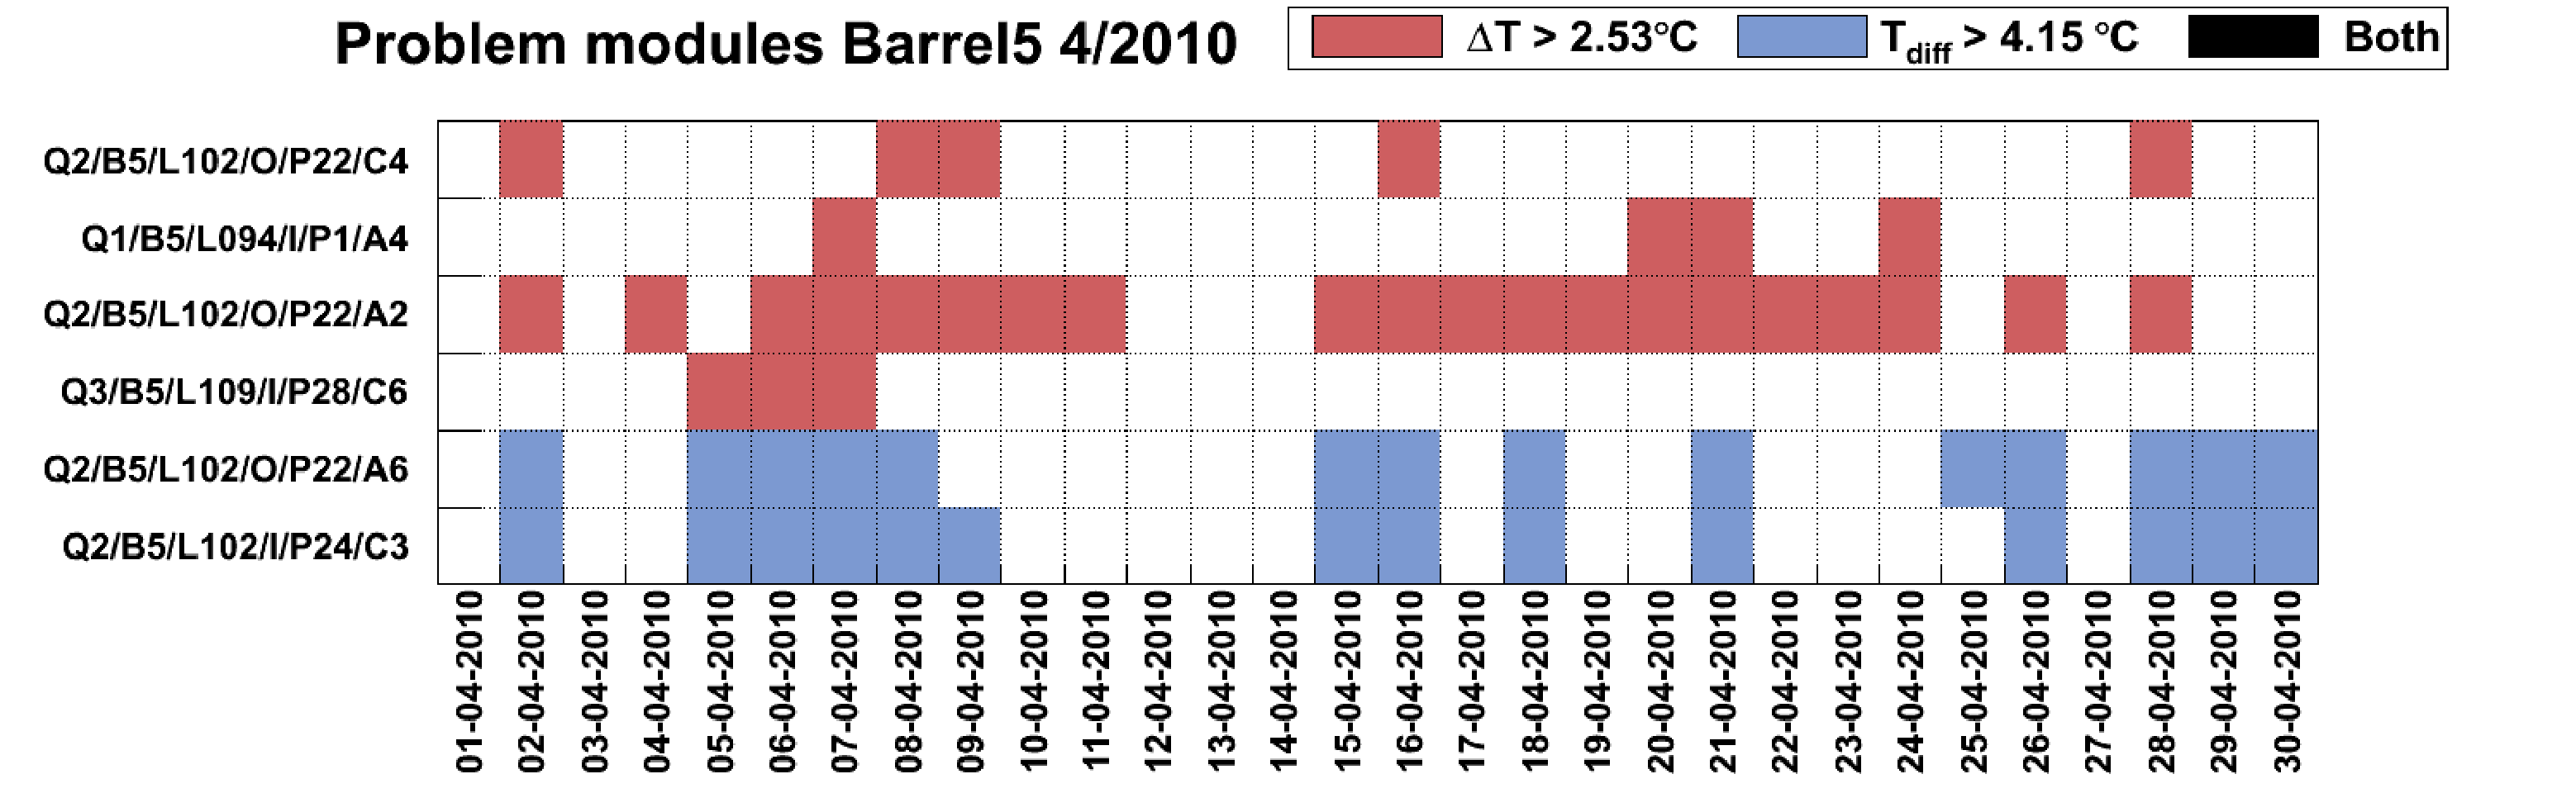
\includegraphics[width=\textwidth]{042010_Barrel5}
	}

	\caption{Problem modules on barrel 5 in April 2010}
	\label{fig:pm_april}
\end{figure}
 
Of obvious concern is whether the number of problematic modules is increasing.
Figure~\ref{fig:num_pm} shows the number of problem modules above threshold on a
given day as a function of time between 20/01/2010 to 16/10/2012 for the \deltat
and \tdiff monitoring variables. For both monitoring varibles, there is no
significant increase in the number of problematic variables observed as a
function of time. Fitting the distributions to a linear function, the average
number of \tdiff modules above the problem threshold is found to increase at a rate
of \NumHighTdiffModulesIncreaseRate\ per year. The average number of \deltat
modules above the problem threshold is found to increase at a rate of
\NumHighDeltaTModulesIncreaseRate\ per year.

\begin{figure}
	\centering
	\subfigure[]{
		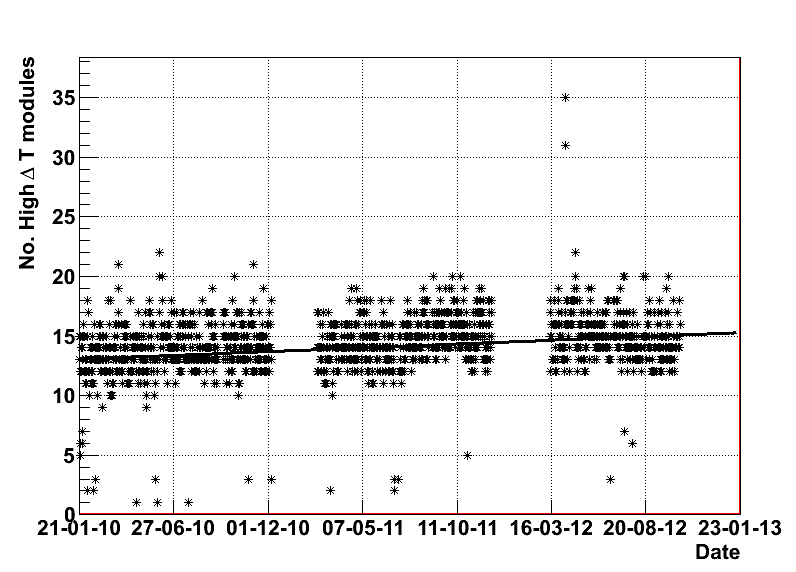
\includegraphics[width=0.47\textwidth]{num_problem_modules/num_high_delta_t}

	}
	\subfigure[]{
		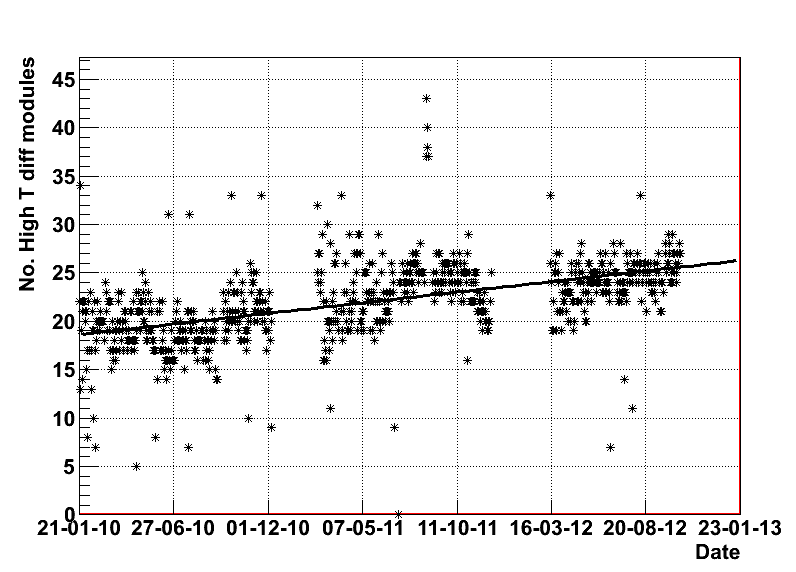
\includegraphics[width=0.47\textwidth]{num_problem_modules/num_high_t_diff}
	}
	\caption{The number of `problematic' modules with (a) \deltat and (b)
        \tdiff of greater magnitude than the problem threshold per day as a
        function of time between 20/01/2010 to 16/10/2012. The number of
        `problematic' modules is not seen to increase significantly as a
        function of time.}
	\label{fig:num_pm}
\end{figure}

\section{Behaviour of problematic modules}

For each of the problematic modules the value of the problematic monitoring variable has been plotted as a function of time for the first six months of 2010 in order to determine whether the problem is getting worse. For most of the problematic modules the magnitude of the monitoring variable does not increase over the period, aside from small fluctuations.  However, one module has been identified with a high \deltat of increasing magnitude, and four modules with a \tdiff of increasing magnitude. A further two show odd behavior. 

\begin{figure}[h]
 	\centering
	\subfigure[]{
		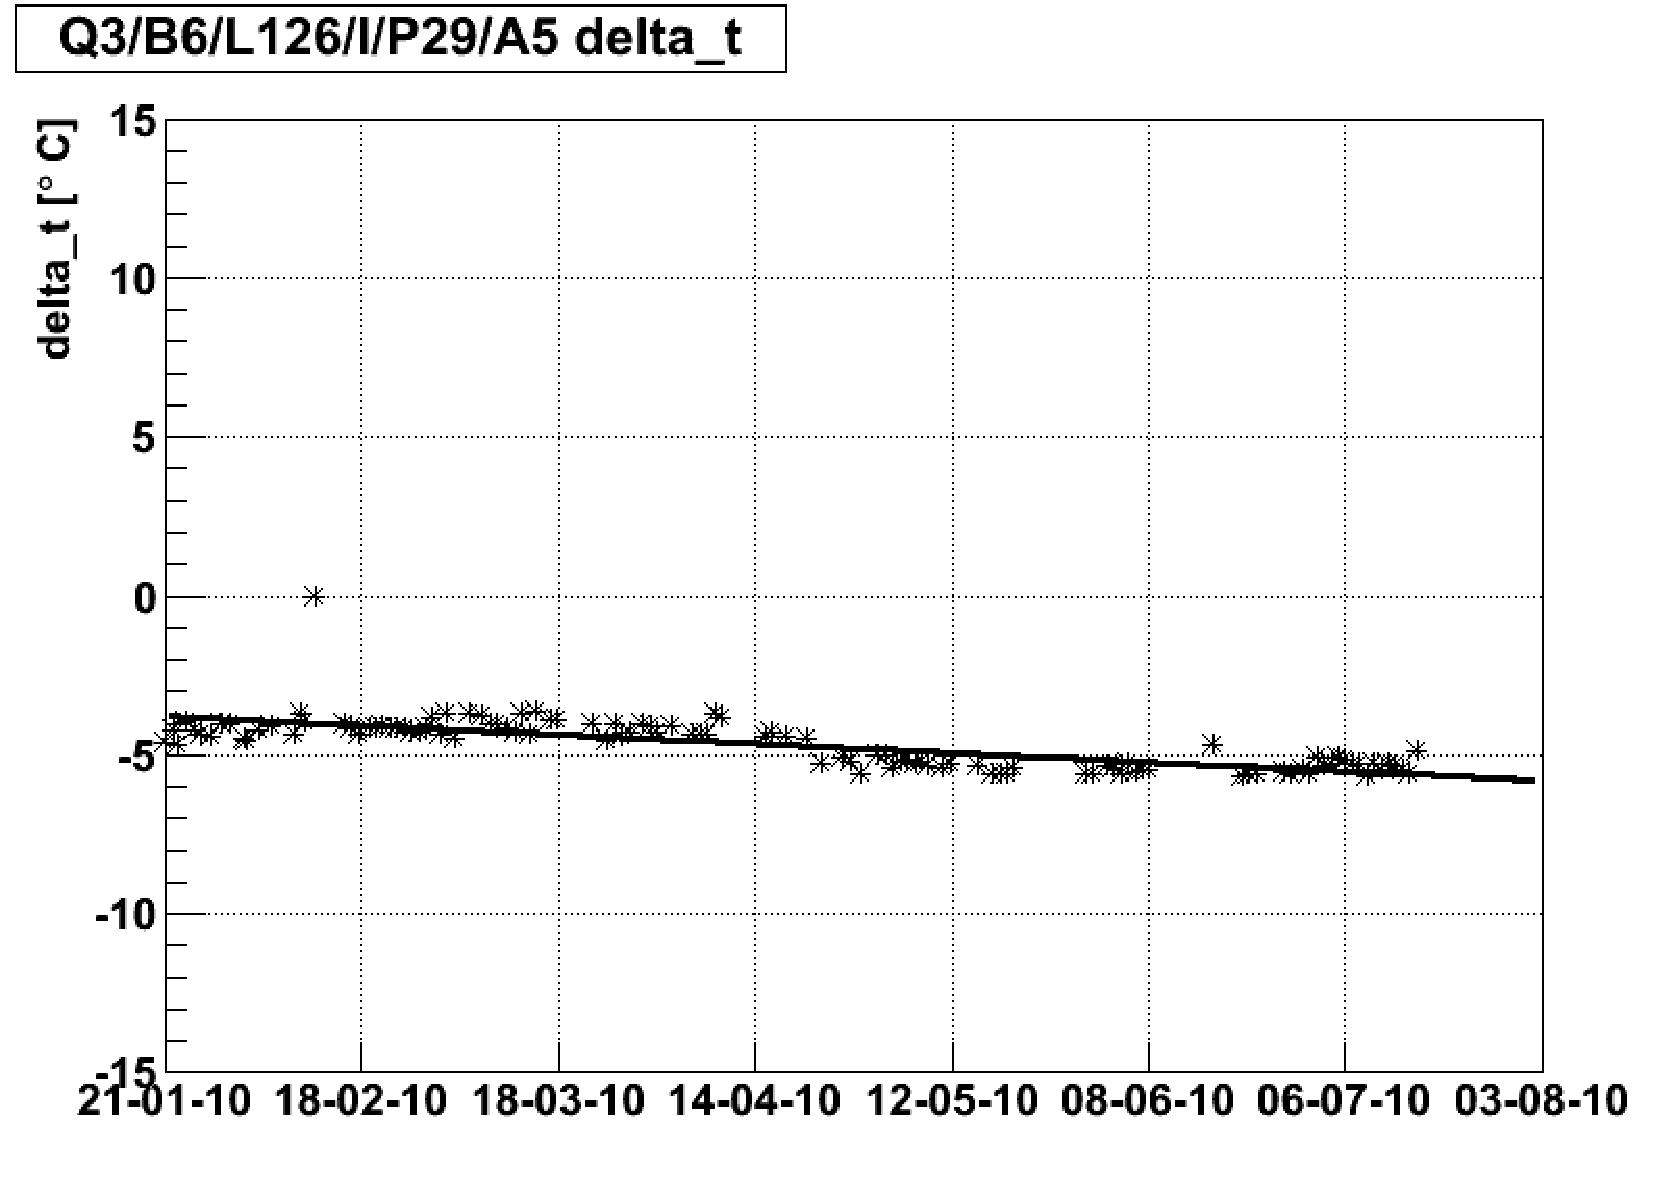
\includegraphics[width=0.47\textwidth]{pm_ev_dt_126-A5}
	}
	\subfigure[]{
		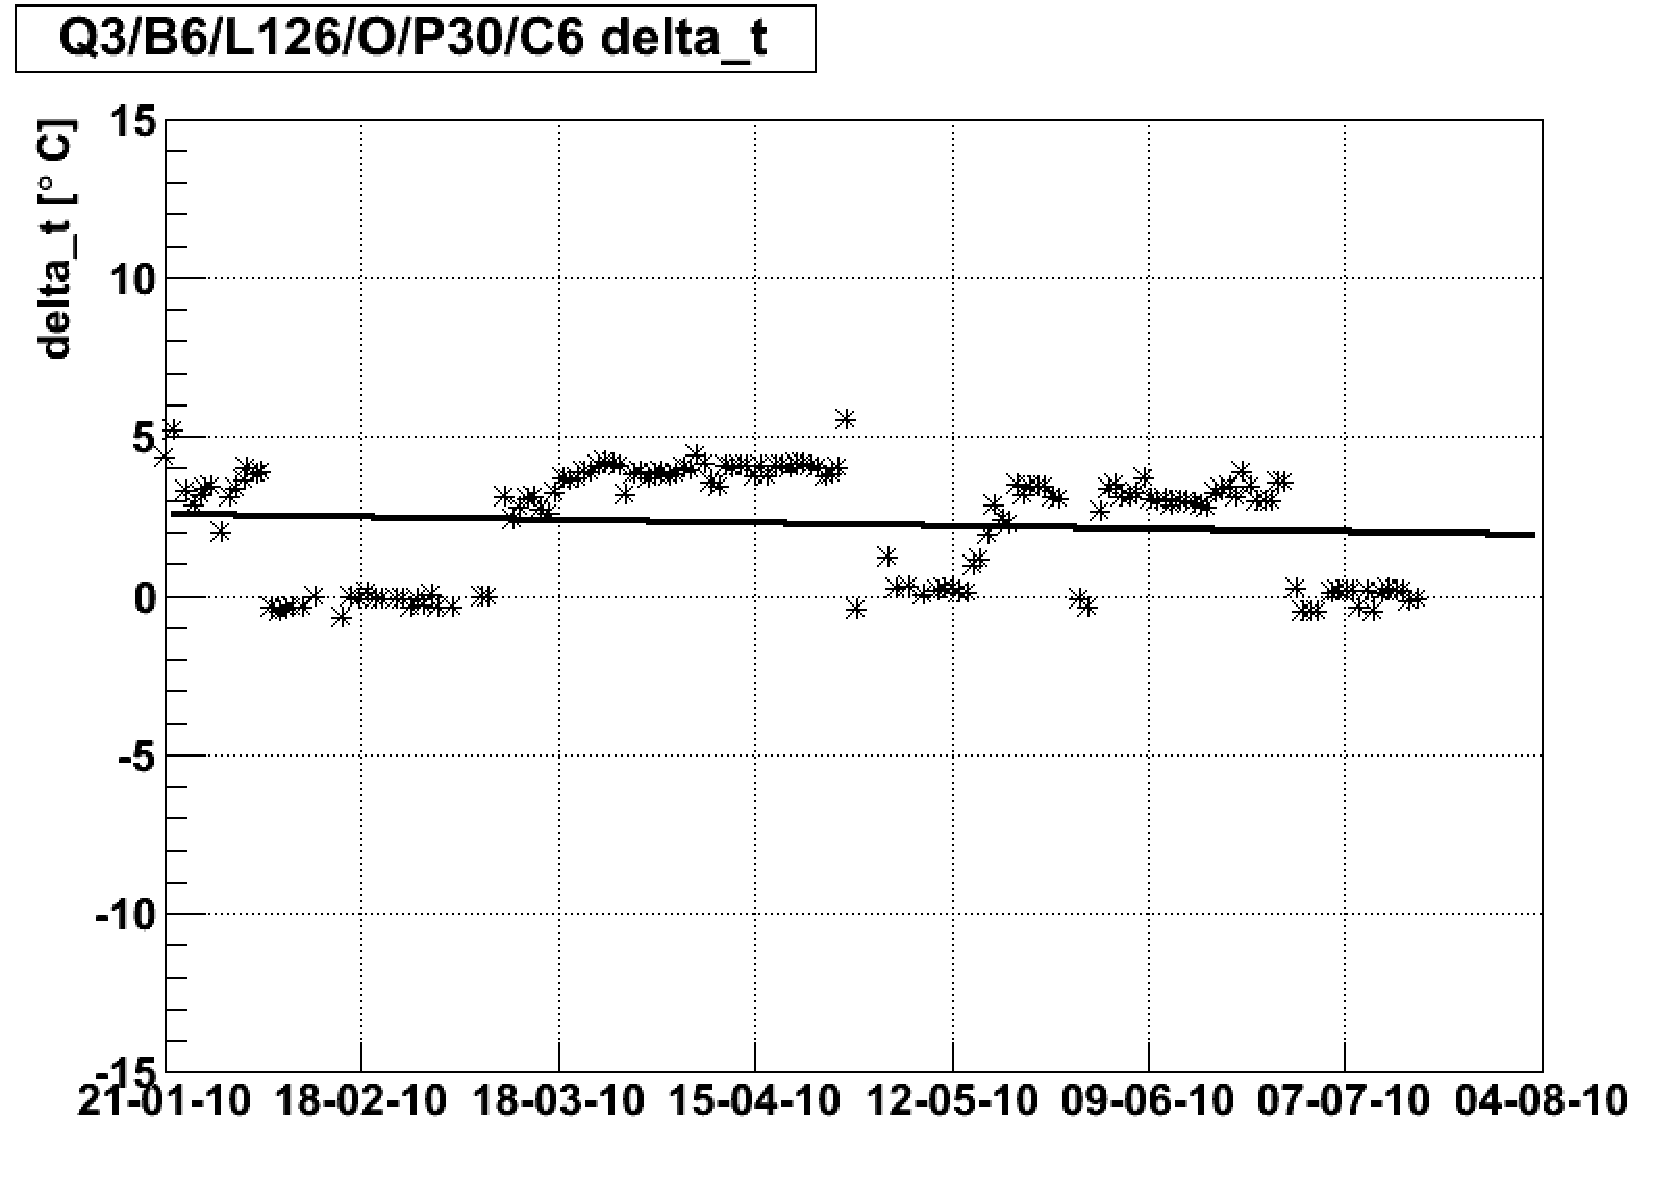
\includegraphics[width=0.47\textwidth]{pm_ev_dt_126-C6}
	}
	\caption{The temperature difference between the front and back of the module (\deltat) for barrel module Q3/B6/L126/I/P29/A5 (left) and barrel module Q3/B6/L126/O/P30/C6 (right) as a function of time between 20/1/2010 to 18/7/2010}
	\label{fig:pm_ev_dt}
\end{figure}

The plot on the left of~\ref{fig:pm_ev_dt} shows the only module with a \deltat of increasing magnitude. The temperature difference between the front and back of the module has increased by about 1.5$^\circ$C in six months, with back of the module warmer than the front. This suggests that the two sides of the module are slowly separating. The plot on the right of~\ref{fig:pm_ev_dt} shows a  module for which \deltat jumps between 0\dc  and 3-4\dc every 1 or 2 months. This suggests an intermittent failure in the integrity of the module, but is very unexpected behaviour and requires further investigation. No other problems with this module have been recorded.

Three modules were observed to have a \tdiff becoming more negative with time, indicating that they are becoming warmer relative to their neighbours by about 1\dc  over six months. This suggests a failure in coupling to the cooling pipe that is getting worse with time. One of these modules is shown on the left of Figure~\ref{fig:pm_ev_tdiff}.  The right hand plot of Figure~\ref{fig:pm_ev_tdiff} shows a module with \tdiff becoming more positive over time, and also showing sharp jumps in the variable. An increasing positive \tdiff means the module is cooler than its neighbours, and becoming even more cooler. This would suggest that the module is running at a lower power, although it is unclear why this would cause the \tdiff to increase over time, nor explain the sudden jumps. Generally modules running at lower power are detected with the DAQ (Data Acquisition) software, but no problem has been reported for this module. A further seven modules with a \tdiff which jumps between 0\dc and around +7 \dc have been observed.  All seven of these modules have other known problems; either the modules do not receive the high voltage, or there is a problem with the module communication. These modules are out of configuration, and data sent from these modules is not used for physics.

\begin{figure}[h]
 	\centering
	\subfigure[]{
		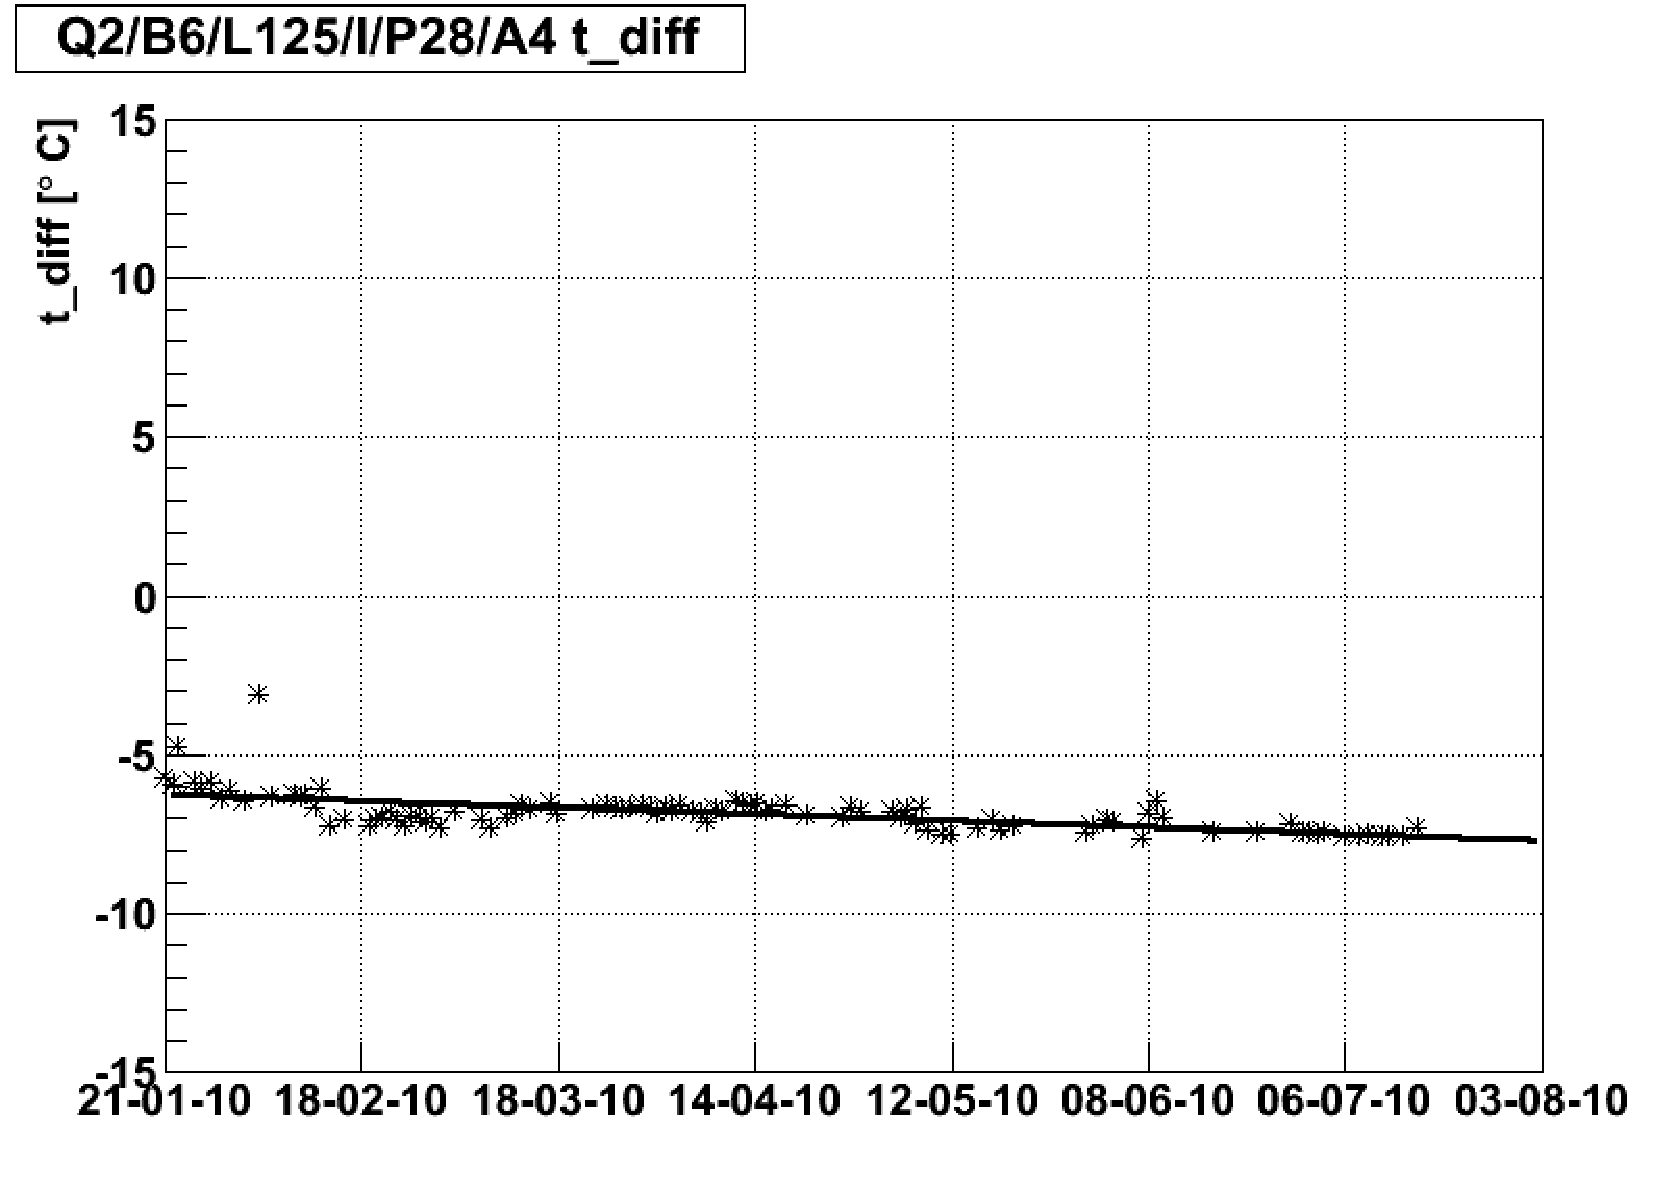
\includegraphics[width=0.47\textwidth]{pm_ev_tdiff_125-A4}
	}
	\subfigure[]{
		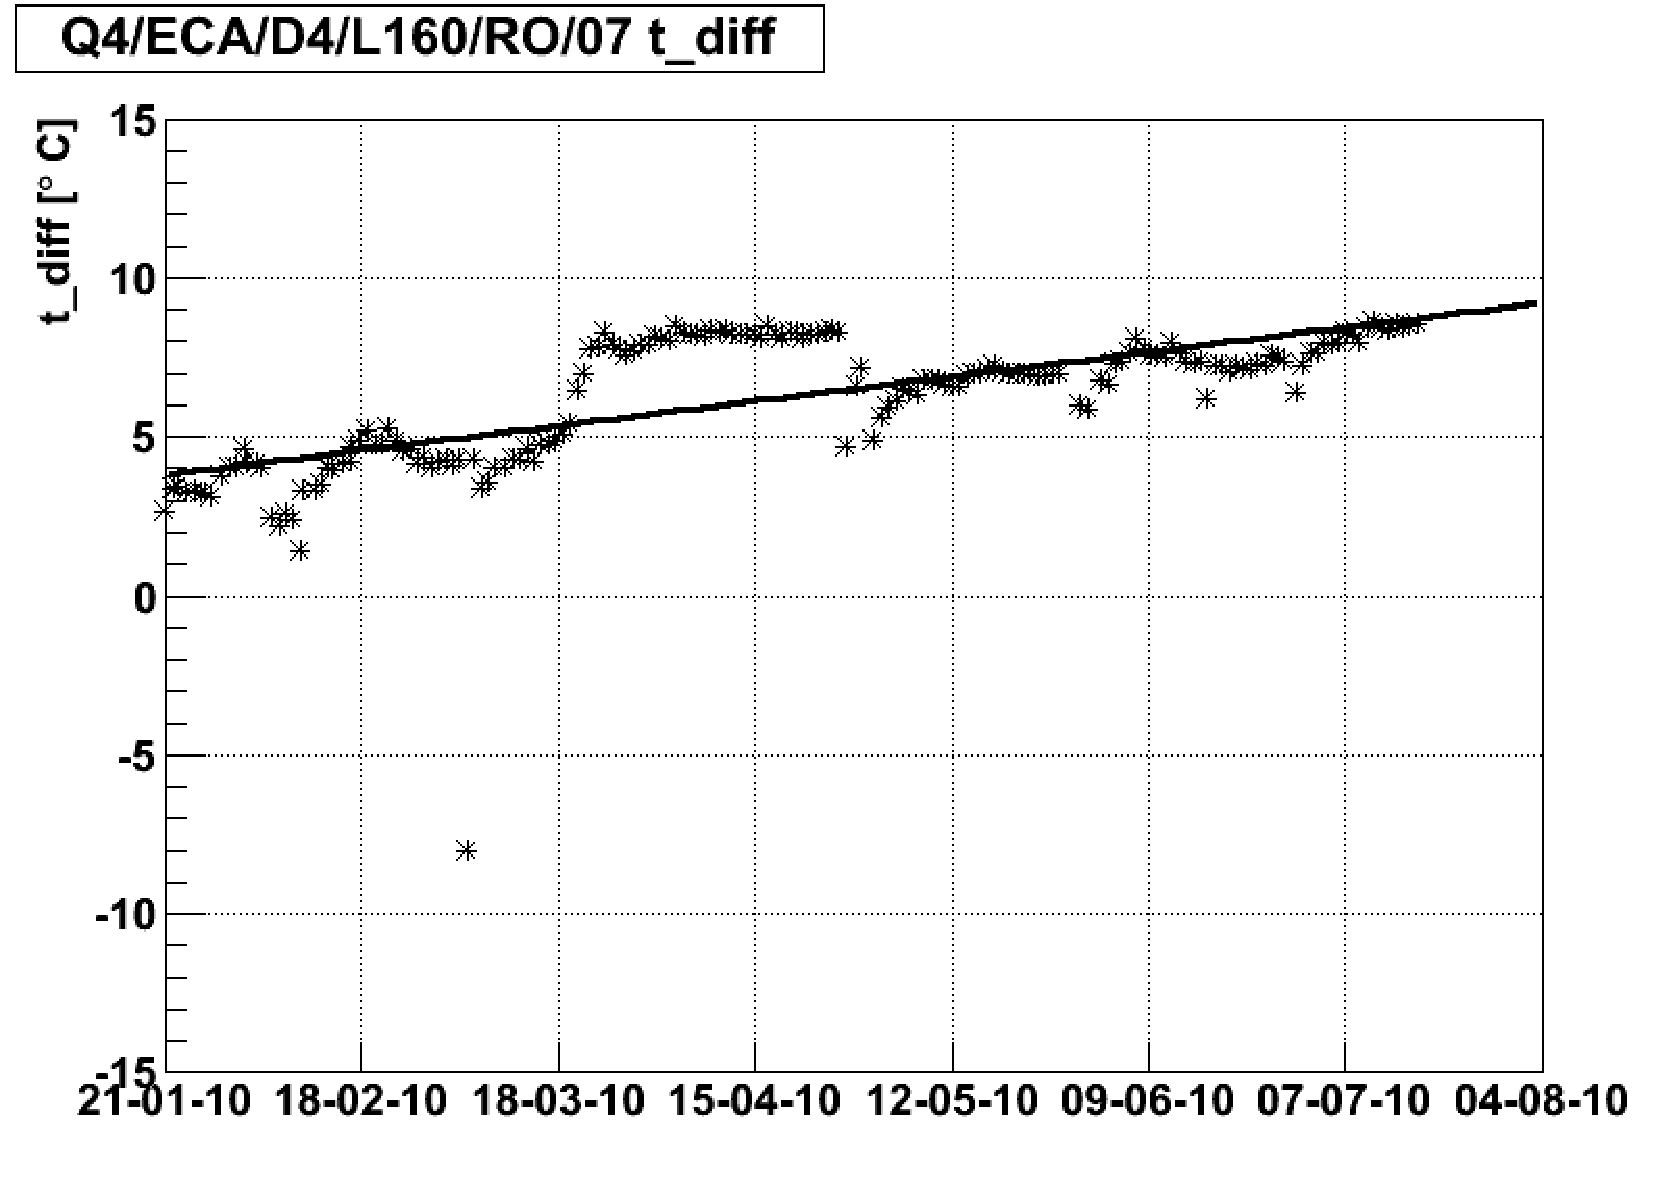
\includegraphics[width=0.47\textwidth]{pm_ev_tdiff_160-07}
	}
	\caption{The difference in temperature between the module and its neighbours (\tdiff) as a function of time for module Q2/B5/L102/I/P24/C3 (left) Q4/ECA/D4/L160/RO/07 (right) between 20/1/2010 to 18/7/2010. }
	\label{fig:pm_ev_tdiff}
\end{figure}

\section{Conclusions}

I plan to cross check problem modules against detector conditions and coincidences with events like powercuts, shutdowns, cooling failures etc, as well as studying characteristics of the individual modules such as the voltage arriving at the module. I also plan to cross check problematic modules against the `production database' which details tests made of modules at production to identify any correlations. 
